%\documentclass{article} % say
%\usepackage{tikz}
%\begin{document}
%We are working on
%\begin{tikzpicture}
%\draw (-1.0,-1.0) -- (1.0,-1.0);
%\draw (-1.0,1.0) -- (1.0,1.0);
%\end{tikzpicture}.
%\end{document
% Author: Till Tantau
% Source: The PGF/TikZ manual
\documentclass{article}

\usepackage[latin1]{inputenc}
\usepackage{tikz}

% GNUPLOT required
\begin{document}
\pagestyle{empty}


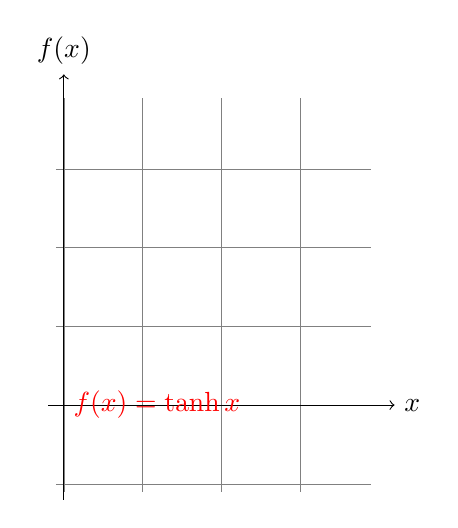
\begin{tikzpicture}[domain=-10:10]
    \draw[very thin,color=gray] (-0.1,-1.1) grid (3.9,3.9);
    \draw[->] (-0.2,0) -- (4.2,0) node[right] {$x$};
    \draw[->] (0,-1.2) -- (0,4.2) node[above] {$f(x)$};
    \draw[color=red] plot[id=tanh] function{atanh(x)} 
        node[right] {$f(x) =\tanh x$};
\end{tikzpicture}


\end{document}}
